
\serie{Simplifier une expression littérale}

\begin{exercice}
Recopie les expressions suivantes en supprimant le signe "$\cdot$" s'il est inutile :
\begin{colitemize}{2}
 \item $A = 9 \cdot n$ ;
 \item $B = x \cdot 3$ ;
 \item $C = 12 \cdot (7 - 3)$ ;
 \item $D = 4 \cdot (3,2 + 6)$ ;
 \item $E = n \cdot x$ ;
 \item $F = 2 \cdot 6$ ;
 \item $G = (3 + 6) \cdot (7 - 1)$ ;
 \item $H = 16 \cdot 3,5 \cdot R$.
 \end{colitemize}
\end{exercice}


\begin{exercice}
Recopie les expressions suivantes en ajoutant le signe "$\cdot$" lorsqu'il est sous-entendu :
\begin{colitemize}{2}
 \item $A = 3x + 2$ ;
 \item $B = ab - 4$ ;
 \item $C = 5(2x - 7)$ ;
 \item $D = 2a(2 + 8)$ ;
 \item $E = 3a - 5b$ ;
 \item $F = ab + 3 \cdot 7a$ ;
 \item $G = b - a + 7(3x + 7)$ ;
 \item $H = a + a - 7b + 1$.
 \end{colitemize}
\end{exercice}


\begin{exercice}
Écris les expressions suivantes le plus simplement possible :
\begin{colitemize}{2}
 \item $A = 3 \cdot a \cdot b$ ; 
 \item $B = 3 \cdot a - 4 \cdot b$ ; 
 \item $C = 8 \cdot a \cdot b \cdot 2$ ;
 \item $D = 3 \cdot (2 \cdot a + b) \cdot 5$ ;
 \item $E = 2 \cdot 3 + 7 - 1$ ;
 \item $F = 2 + 5 + 3 \cdot b$ ; 
 \item $G = (2,5 - 1) \cdot a \cdot b$ ; 
 \item $H = 2 \cdot 3 \cdot a \cdot (b \cdot c)$.
 \end{colitemize}
\end{exercice}


\begin{exercice}
Écris les expressions suivantes le plus simplement possible en utilisant les notations "au carré" et "au cube" si nécessaire :
\begin{colitemize}{2}
 \item $A = 1 \cdot a + a \cdot a$ ;
 \item $B = a \cdot a \cdot a - 0 \cdot b$ ;
 \item $C = 6 \cdot a \cdot a - a$ ; 
 \item $D = 2 \cdot a \cdot 3 \cdot a$ ; 
 \item $E = a \cdot a \cdot b \cdot 3$ ;
 \item $F = 1 \cdot a \cdot a \cdot b \cdot 0$ ;
 \item $G = a \cdot 2 \cdot b \cdot a \cdot b$ ;
 \item $H = (a + b) \cdot (a + b)$.
 \end{colitemize}
Aire d'un carré de côté $c$ : $c \cdot c = \ldots$
\end{exercice}


\begin{exercice}
Traduis par une expression littérale les phrases suivantes :
\begin{enumerate}
 \item La somme de $x$ et de 13 ;
 \item Le double de $x$ ;
 \item La différence de $x$ et de 7 ;
 \item Le tiers de $x$ ;
 \item Le triple de la somme de 2 et de $x$ ;
 \item Le tiers de la différence entre 16 et $x$.
 \end{enumerate}
\end{exercice}


\begin{exercice}
Calcule les expressions suivantes pour les valeurs de $x$ et de $y$ indiquées :
\begin{colitemize}{2}
 \item $A = 4 x + 3$ ;
 \item $B	= 3 x^2$ ;
 \item $C	= x y - x - y + 4$ ;
 \item $D	= x^2 + 2xy + y^2$ ;
 \item $E	= x^2 + y^2$ ;
 \item $F	= x^2 y$.
 \end{colitemize}
 \begin{enumerate}
  \item Pour $x = 2$ et $y = 3$ ;
  \item Pour $x = 3$ et $y = x$.
  \end{enumerate}
\end{exercice}

%%%%%%%%%%%%%%%%%%%%%%%%%%%%%%%%%%%%%%%%%%%%%%%%%%%%%%%%%%%%%%%%%%%%%%%%%

\serie{Produire une expression littérale}

\begin{exercice}[Périmètres]
\begin{enumerate}
 \item Exprime le périmètre des figures ci-dessous en fonction de $a$ et de $b$ sachant qu'un trait bleu mesure $a$ cm, un trait rose mesure $2a$ cm et un trait vert mesure $b$ cm :
 
\begin{minipage}[c]{0.48\linewidth}
 \begin{center} 
\includegraphics[width=2.5cm]{perimetre1} \end{center}
 \end{minipage} \hfill%
 \begin{minipage}[c]{0.48\linewidth}
  \begin{center} 
\includegraphics[width=2.9cm]{perimetre2} \end{center} 
  \end{minipage} \\
 \item Calcule ensuite ces deux périmètres pour $a = 1,3$ et $b = 4$.
 \end{enumerate}
\end{exercice}


\begin{exercice}[Aire en fonction de $x$]
\begin{minipage}[c]{0.48\linewidth}
 \begin{enumerate}
  \item Calcule l'aire de la partie coloriée en fonction de $x$.
  \item Combien vaut cette aire si $x = 14,7 \text{m}$ ?
  \end{enumerate}
 \end{minipage} \hfill%
 \begin{minipage}[c]{0.48\linewidth}
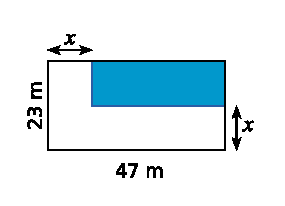
\includegraphics[width=4.1cm]{aire_fx}
  \end{minipage} \\
\end{exercice}


\begin{exercice}
Pour son téléphone portable, Grégoire paye : 12 CHF d'abonnement, $a$ CHF par SMS envoyé et 40 centimes par minute de communication. 
\begin{enumerate}
 \item Écris une expression permettant de calculer sa dépense sachant que ce mois-ci, Grégoire a envoyé 30 SMS et a utilisé $m$ minutes de communications.
 \item Quelle est cette dépense si $a = 0,8$ et $m = 150$ ?
 \end{enumerate}
\end{exercice}


\begin{exercice}
Sandrine a construit un triangle tel que la longueur d'un petit côté vaut la moitié de celle du grand et la longueur du moyen vaut les trois quarts de celle du grand.
\begin{enumerate}
 \item Écris une expression permettant de calculer le périmètre du triangle en fonction de la longueur $L$ du plus grand des côtés ;
 \item Détermine le périmètre si $L$ vaut 7 cm.
 \end{enumerate}
\end{exercice}


%%%%%%%%%%%%%%%%%%%%%%%%%%%%%%%%%%%
%%%%%%%%%%%%%%%%%%%%%%%%%%%%%%%%%%%
%MiseEnPage
%%%%%%%%%%%%%%%%%%%%%%%%%%%%%%%%%%%
\newpage
%%%%%%%%%%%%%%%%%%%%%%%%%%%%%%%%%%%
%%%%%%%%%%%%%%%%%%%%%%%%%%%%%%%%%%%

\begin{exercice}
Marc a rentré trois nombres en mémoire dans sa machine à calculer. Pour cela, il a utilisé les lettres $a$, $b$ et $c$. Il veut maintenant calculer les expressions suivantes :
\begin{itemize}
 \item $S = 2a - 3b + 7c + 5$ ;
 \item $T = 7ab + 4c - 8$.
 \end{itemize}
Calcule ces expressions pour $a = 12$, $b = 5$ et $c = 7$. Vérifie les résultats obtenus à l'aide de ta calculatrice.
\end{exercice}


\begin{exercice}
Exprime en fonction de $x$ et $y$ les périmètres du carré et du rectangle suivants :
\begin{center} 
\includegraphics[width=4.3cm]{rectangles_xy} \end{center} 
Pour les valeurs de $x$ et de $y$ suivantes, le périmètre du carré est-il supérieur à celui du rectangle ?
\begin{colenumerate}{2}
 \item $x = 2$ et $y = 1$ ; 
 \item $x = 3$ et $y = 1$ ; 
 \item $x = 6$ et $y = 3$ ; 
 \item $x = 10$ et $y = 7$.
 \end{colenumerate}
\end{exercice}


\begin{exercice}[La grande bleue]
\begin{center} 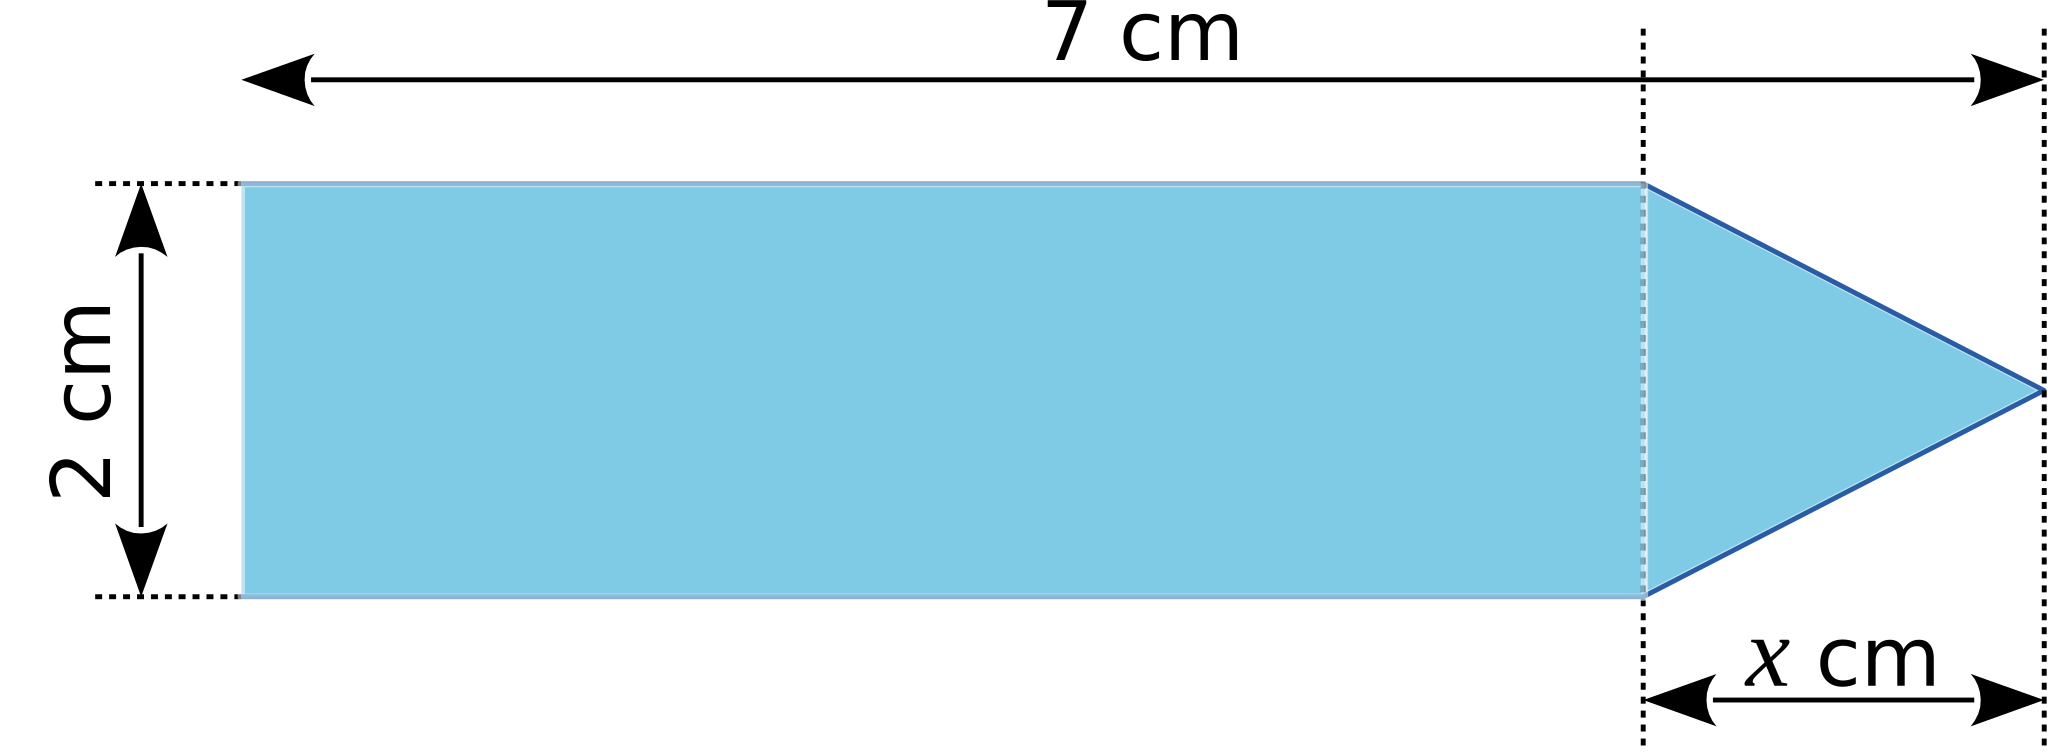
\includegraphics[width=8.1cm]{grande_bleue} \end{center}
\begin{enumerate}
 \item Exprime l'aire de la surface bleue en fonction de $x$ ;
 \item Calcule cette aire pour $x = 3 cm$.
 \end{enumerate}
\end{exercice}


\begin{exercice}
Marie dit qu'en ajoutant deux nombres impairs, on obtient toujours un nombre impair :
\begin{enumerate}
 \item Prouve-lui qu'elle a tort à l'aide d'un contre-exemple ;
 \item En utilisant la variable $n$, écris une expression désignant un nombre pair puis une autre désignant un nombre impair ; \label{CalcLit_entrain1}
 \item Utilise la question \ref{CalcLit_entrain1} pour démontrer à Marie que la somme de deux nombres impairs n'est jamais impaire.
 \end{enumerate}
\end{exercice}


\begin{exercice}
Vanessa a acheté un cahier à 2 CHF et trois classeurs à $x$ CHF :
\begin{enumerate}
 \item Exprime le prix total qu'elle a payé en fonction de $x$ ;
 \item Elle a payé 23 CHF en tout. Retrouve le prix d'un classeur.
 \end{enumerate}
\end{exercice}


\begin{exercice}[Un carré qui grandit]
Soit $ABCD$ un carré de 5 cm de côté :
\begin{enumerate}
 \item Calcule le périmètre et l'aire de $ABCD$.
 \end{enumerate}
On augmente son côté de $k$ cm. Exprime, en fonction de $k$ :
\begin{enumerate}
\setcounter{enumi}{1}
 \item La longueur $L$ de ce nouveau côté ;
 \item Le nouveau périmètre $P$ de ce carré ;
 \item La nouvelle aire $S$ de ce carré ;
 \item L'augmentation $A_p$ du périmètre ;
 \item L'augmentation $A_s$ de l'aire.
 \end{enumerate}
\end{exercice}
